\documentclass[11pt,a4paper]{article}
\usepackage[utf8]{inputenc}
\usepackage[spanish]{babel}	%Idioma
\usepackage{amsmath}
\usepackage{url}
\makeatletter
\makeatother
\usepackage{amsfonts}
\usepackage{amssymb}
\usepackage{graphicx} 	%Añadir imágenes
\usepackage{geometry}	%Ajustar márgenes
\usepackage[export]{adjustbox}[2011/08/13]
\usepackage{float}
\restylefloat{table}
\usepackage[hidelinks]{hyperref}
\usepackage{titling}
\graphicspath{}
\usepackage{multirow}
\usepackage{caption}
\usepackage{multicol}
\usepackage{array}
\usepackage{eurosym}


%Opciones de encabezado y pie de página:
\usepackage{fancyhdr}
\pagestyle{fancy}
\lhead{Grado en Ingeniería Informática}
\rhead{Descripción de la Aplicación}
\lfoot{Sistemas Gráficos}
\cfoot{}
\rfoot{\thepage}
\renewcommand{\headrulewidth}{0.4pt}
\renewcommand{\footrulewidth}{0.4pt}

%Opciones de fuente:
\usepackage[utf8]{inputenc}
\usepackage[default]{sourcesanspro}
\usepackage{sourcecodepro}
\usepackage[T1]{fontenc}

\setlength{\parindent}{15pt}
\setlength{\headheight}{15pt}
\setlength{\voffset}{10mm}

% Custom colors
\usepackage{color}
\definecolor{deepblue}{rgb}{0,0,0.5}
\definecolor{deepred}{rgb}{0.6,0,0}
\definecolor{deepgreen}{rgb}{0,0.5,0}
\hypersetup{
    colorlinks=true,
    linkcolor=black,
    urlcolor=blue,
}

\usepackage{listings}

\begin{document}
\sloppy
\begin{titlepage}
  \centering
  
\includegraphics[width=0.7\textwidth]{logo.png}\par\vspace{1cm}
  {\scshape\large Sistemas Gráficos \par} \vspace{1cm}
  {\huge\bfseries Diseño e implementación de \\ un sistema gráfico \par}
  \vspace{0.4cm}
  {\large\bfseries ---Descripción---\\}
  \vspace{0.6cm}
  {\large\itshape  Guillermo Sandoval Schmidt  \par} \vspace{1.00cm}
  Curso 2019-2020 \\
  \vfill

  % Bottom of the page
  {\large \today\par}
\end{titlepage}

\pagenumbering{gobble}
\pagenumbering{arabic}
\tableofcontents
\thispagestyle{empty}

\newpage

\section{Grupo de prácticas}
\begin{itemize}
    \item \textbf{Nombre de Alumno:} Guillermo Sandoval Schmidt
    \item \textbf{Nombre de la Aplicación:} Tetris
\end{itemize}


\section{Descripción}

\begin{multicols}{2}

La aplicación que se quiere desarrollar e implementar está inspirada en el juego 'Tetris'. El juego consiste en una serie de piezas con diversas formas, compuestas de 4 cubos cada una que caen por la pantalla, quedando apiladas hasta llegar a la parte superior de la pantalla, siendo ese el fin de la partida. El jugador puede mover horizontalmente las piezas, hacer que caigan más rápido y girar estas en ambos sentidos, tanto izquierda como derecha. Cuando el jugador completa una línea horizontal, esta desaparece, creando espacio nuevo y haciendo que el resto de piezas acumuladas desaparezcan. 

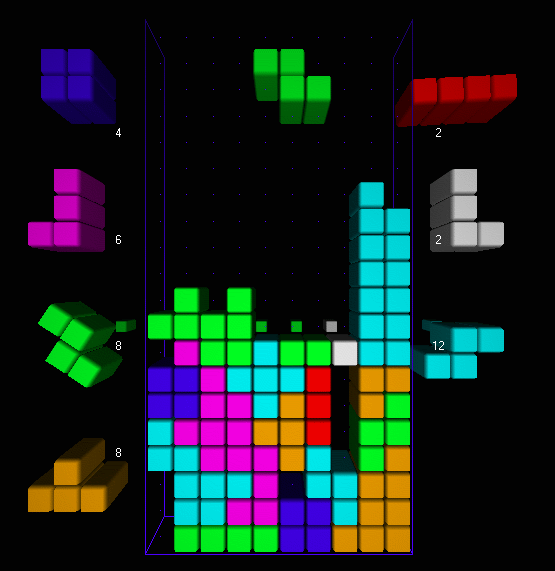
\includegraphics[scale=0.32]{tetris.png}

\end{multicols}

\subsection{Funcionalidad mínima}

\begin{itemize}
    \item \textbf{Tablero de juego.} El tablero de juego es una matriz compuesta por X*Y cubos. 
    \item \textbf{Piezas.} Se implementarán 7 piezas distintas, con las formas clásicas del juego 'Tetris'.
    \item \textbf{Interfaz auxiliar.} El juego cuenta con una interfaz auxiliar que nos muestra la próxima pieza que va a caer y una pieza que podremos reservar.
    \item \textbf{Controles.} Se implementarán los controles con el teclado.
    \item \textbf{Gravedad.} El proyecto contendrá un sistema de 'gravedad' que haga que las piezas caigan una posición cada X segundos.
    \item \textbf{Colisiones.} Hace falta implementar un sistema de detección de colisiones para que 1) no permita girar piezas si la posición resultante supone una colisión entre dos piezas o si se sale del tablero y 2) permita 'fijar' las piezas al colisionar con la parte inferior del tablero o con las piezas ya 'bloqueadas'.
    \item \textbf{Mecánicas de juego.} Cuando se forma una línea en el tablero, esta desaparecerá y todas las piezas ya 'situadas' por encima de la línea que desaparezca caerán una posición.
\end{itemize}

\subsection{Funcionalidad extra}

\begin{itemize}
    \item \textbf{Puntuación.} Cuando se forme 1,2,3 o 4 líneas simultáneamente, el jugador obtendrá puntos que se sumarán a su puntuación total.
    \item \textbf{Modo 2 jugadores.} Este modo tiene varias implicaciones:
        \begin{itemize}
            \item \textbf{Doble pantalla.} Habrá dos partidas en paralelo, una controlada por cada jugador con su configuración de teclas.
            \item \textbf{Mecánicas de juego.} Cuando un jugador elimina X líneas, estas aparecen en la pantalla del rival, provocando que se llene el tablero del rival.
        \end{itemize}
    \item \textbf{Menú de inicio.} Si da tiempo, se implementará un menú de inicio con una pequeña animación y que permita elegir modo de juego, cambiar los controles, etc.
\end{itemize}

\section{Interacción}

La interacción con las piezas será mediante teclado y tendrá que tener teclas asociadas a:

\begin{itemize}
    \item Movimiento horizontal, hacia la derecha y hacia la izquierda.
    \item Movimiento vertical. Solo movimiento descendente.
    \item Caída libre. Hará que la pieza caiga de golpe.
    \item Reservar pieza.
\end{itemize}

Además sería interesante incluir una tecla que pause la partida.

En caso de implementar el menú inicial, la interacción con el mismo será tanto con el ratón como con el teclado.

\end{document}
